\section{Zielsetzung}
Dieser Versuch fokusiert sich auf die Untersuchung einer Wärmepumpe und Ermittlung der Qualität dieser.
\section{Theorie}
\label{sec:Theorie}
Der zweite Hauptsatz der Thermodynamik besagt, dass Wärmeenergie vom wärmeren in das kältere Reservoir fließt.
Damit sich die Flussrichtung der Wärmeenergie ändert muss beispielsweise mechanische Arbeit aufgewendet werden.
Eine Apparatur, welche dieses vollführt, ist die Wärmepume.
Der erste Hauptsatz der Thermodynamik besagt:
\begin{equation}
	\symup{\Delta} U = \symup{\Delta} Q + \symup{\Delta} A
\end{equation}
Für die Wärmepumpe folgt daraus, dass
\begin{equation}
	\label{eq:herleitung1}
	Q_1 = Q_2 + A
\end{equation}
gelten muss.
Die Güteziffer
%
\begin{equation}
	\label{eq:gl1}
	\nu=\frac{Q_1}{A}
\end{equation}
%
beschreibt das Verhältnis zwischen transportierter Wärmemenge und verrichteter Arbeit.
Mit dem zweiten Hauptsatz der Thermodynamik lässt sich nun folgende Aussage über Wärmemengen der beiden Reservoirs und Temperaturen dieser treffen:
\begin{equation}
		\label{eq:gl2}
	\frac{Q_1}{T_1}-\frac{Q_2}{T_2}=0.
\end{equation}
Dies gilt jedoch nur unter den idealisierten Bedingungen, dass der Prozess reversibel ist.
Aus Gleichung \eqref{eq:herleitung1} und \eqref{eq:gl2} folgt:
\begin{equation}
	Q_1 = A + \frac{T_2}{T_1} Q_2 .
\end{equation}
Somit lässt sich die ideale Güteziffer durch
\begin{equation}
	\nu_{\text{id}}=\frac{T_1}{T_1-T_2}.
	\label{eq:guetezifferideal}
\end{equation}
beschreiben.
Daraus ist erkennbar, dass die Wärmepumpe um so effizienter arbeitet je kleiner die Temperaturdifferenz zwischen den Wärmereservoirs ist.
Die reale Wärmepumpe kann diese Forderung jedoch nicht erfüllen.
Für den realen, irreversiblen Fall gilt
\begin{equation}
		\label{eq:gl3}
	\frac{Q_1}{T_1}-\frac{Q_2}{T_2}>0
\end{equation}
und damit für die reale Güteziffer:
\begin{equation}
\nu_{\text{real}} < \frac{T_1}{T_1-T_2}
\end{equation}
\subsection{Aufbau der Wärmepumpe}
\label{sec:AdW}
In Abbildung \ref{fig:aufbau} wird der Aufbau einer Wärmepumpe dargestellt.
Innerhalb eines geschlossenen Systems verdampft und kondensiert ein Gas in den verschiedenen Wärmereservoirs.
Dies wird durch Druckunterschiede in den Wärmereservoirs realisiert.
Das Gas wird komprimiert wodurch es kondensiert und Wärme an das Reservoir 1 abgibt.
Das Transportmedium durchläuft das Drosselventil D und geht in dem Reservoir 2 in Gasform über.
Hierbei entzieht es Reservoir 2 Wärme.
In dem flüssigen Zustand wird das Transportmedium von Gasresten mittels eines "Reinigers" befreit, um die Funktion des
Drosselventils zu gewährleisten.
Dieses wird so geregelt, dass keine Flüssigkeit in den Kompressor gelangt, da dies den Kompressor beschädigen kann.
\begin{figure}[H]
    \centering
    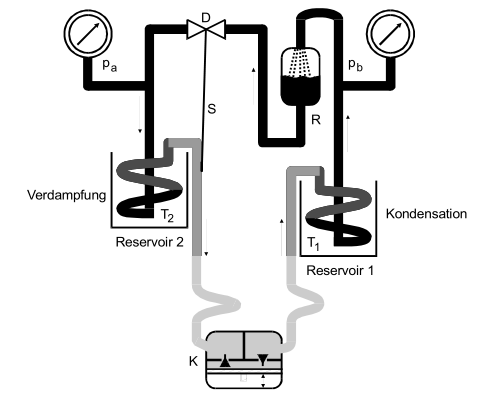
\includegraphics[width=\textwidth]{content/aufbau.png}
    \caption{Aufbau der Wärmepumpe\cite{v206}}
    \label{fig:aufbau}
\end{figure}
\subsection{Bestimmung der Kenngrößen}
\label{sec:BdK}
Die Güteziffer, der Massendurchsatz des Transportmediums und Wirkungsgrad des Kompressors sind in diesem Versuch die
interessanten Kenngrößen.
Die pro Zeiteinheit gewonnene Wärmemenge berechnet sich nach:
\begin{equation}
	\frac{\symup{d}Q_1}{\symup{dt}}=(m_1c_{\text{w}}+m_{\text{k}}c_{\text{k}}) \frac{\symup{d}T_1}{\symup{dt}}.
	\label{eq:gueteziffer}
\end{equation}
Hierbei sind $c_{\text{w}}$ und $c_{\text{k}}$ die Wärmekapazität des Wassers und der Apparatur.
Mit der Leistungsaufnahme $A$ lässt sich die Güteziffer durch
\begin{equation}
	\nu=\frac{1}{A}\frac{\symup{d}Q_1}{\symup{dt}}
    \label{eq:leistung}
\end{equation}
beschreiben.
Analog zu \eqref{eq:gueteziffer} lässt sich die entnommene Wärmemenge $Q_2$ pro Zeiteinheit bestimmen.
Ist die Verdampfungswärme $L$ bekannt, kann der Massendurchsatz
\begin{equation}
	\frac{\symup{d}m}{\symup{dt}}=\frac{1}{L}\frac{\symup{d}Q_2}{\symup{dt}}
	\label{eq:massendurchsatz}
\end{equation}
berechnet werden.
Die mechanische Kompressorleistung berechnet sich über:
\begin{equation}
	N_{\text{mech}} = \frac{1}{\kappa - 1} \left( p_{\text{b}}
        \sqrt[{\leftroot{-1}\uproot{2}\kappa}]{
        \frac{p_{\text{a}}}{p_{\text{b}}}} -p_{\text{a}}\right)
        \frac{1}{\rho}
        \frac{\symup{d}m}{\symup{dt}}.
	\label{eq:arbeit}
\end{equation}
Wobei $\rho$ die Dichte des Transportmediums bezeichnet.
